
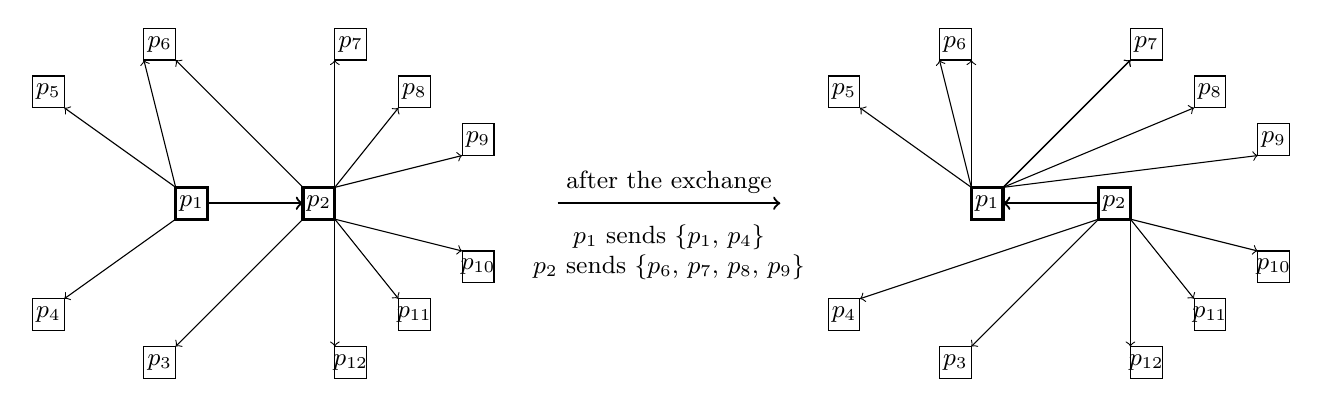
\begin{tikzpicture}[scale=1.15]
  \small

  \draw[->] (-5pt,  5pt) -- ( -40pt,  30pt );
  \draw[->] (-5pt,  -5pt) -- ( -40pt, -30pt );
  \draw[->] (-5pt,  5pt) -- ( -15pt,  45pt );

  \draw[->, thick] (5pt, 0pt) -- (35pt, 0pt);
  \draw[->] (35pt, -5pt) -- (-5pt, -45pt);
  \draw[->] (35pt, 5pt) -- (-5pt, 45pt);

  \draw[fill=white, very thick](0pt, 0pt)
  node{$p_1$}+(-5pt,-5pt)rectangle +(5pt,5pt);
  \draw[fill=white] (-10pt, 50pt)node{$p_6$} +(-5pt,-5pt) rectangle +(5pt,5pt);
  \draw[fill=white] (-45pt, 35pt)node{$p_5$} +(-5pt,-5pt) rectangle +(5pt,5pt);
  \draw[fill=white] (-45pt,-35pt)node{$p_4$} +(-5pt,-5pt) rectangle +(5pt,5pt);
  \draw[fill=white] (-10pt,-50pt)node{$p_3$} +(-5pt,-5pt) rectangle +(5pt,5pt);

  \begin{scope}[shift={(40pt,0pt)}]
  \draw[->] (5pt, -5pt) -- (   5pt, -45pt );
  \draw[->] (5pt, -5pt) -- ( 45pt, -15pt );
  \draw[->] (5pt, -5pt) -- ( 25pt, -30pt );
  \draw[->] (5pt, 5pt) -- (  25pt, 30pt );
  \draw[->] (5pt, 5pt) -- (  45pt, 15pt );
  \draw[->] (5pt, 5pt) -- (   5pt, 45pt );

  \draw[fill=white, very thick] (0pt, 0pt)
  node{$p_2$} +(-5pt,-5pt) rectangle +(5pt,5pt);
  \draw[fill=white] ( 10pt, 50pt)node{$p_{7}$}+(-5pt,-5pt)rectangle+(5pt,5pt);
  \draw[fill=white] ( 30pt, 35pt)node{$p_{8}$}+(-5pt,-5pt)rectangle+(5pt,5pt);
  \draw[fill=white] ( 50pt, 20pt)node{$p_{9}$}+(-5pt,-5pt)rectangle+(5pt,5pt);

  \draw[fill=white] ( 50pt,-20pt)node{$p_{10}$}+(-5pt,-5pt)rectangle+(5pt,5pt);
  \draw[fill=white] ( 30pt,-35pt)node{$p_{11}$}+(-5pt,-5pt)rectangle+(5pt,5pt);
  \draw[fill=white] ( 10pt,-50pt)node{$p_{12}$}+(-5pt,-5pt)rectangle+(5pt,5pt);
  \end{scope}
 

  \draw[->,thick] (115pt, 0pt) --node[anchor=south]{after the exchange}
  node[anchor=north, align=center]{ \ \\
    $p_1$ sends $\left\{p_1,\,p_4\right\}$\\
  $p_2$ sends $\left\{p_6,\,p_7,\,p_8,\,p_9\right\}$}
  (185pt, 0pt);

  \begin{scope}[shift={(250pt, 0pt)}]
  \draw[->] (-5pt,  5pt) -- ( -40pt,  30pt );
  \draw[->] (-5pt,  5pt) -- ( -15pt,  45pt );
  \draw[->] (-5pt,  5pt) -- (  -5pt,  45pt );
  \draw[->] ( 5pt,  5pt) -- ( 45pt, 45pt);

  \draw[<-, thick] (5pt, 0pt) -- (35pt, 0pt);
  \draw[->] (35pt, -5pt) -- (-5pt, -45pt);
  \draw[->] (35pt, -5pt) -- (-40pt, -30pt);
  \draw[->] (5pt, 5pt) -- (  45pt, 45pt );
  \draw[->] (5pt, 5pt) -- ( 85pt,  15pt );
  \draw[->] (5pt, 5pt) -- ( 65pt,  30pt );

  \draw[fill=white, very thick](0pt, 0pt)
  node{$p_1$}+(-5pt,-5pt)rectangle +(5pt,5pt);
  \draw[fill=white] (-10pt, 50pt)node{$p_6$} +(-5pt,-5pt) rectangle +(5pt,5pt);
  \draw[fill=white] (-45pt, 35pt)node{$p_5$} +(-5pt,-5pt) rectangle +(5pt,5pt);
  \draw[fill=white] (-45pt,-35pt)node{$p_4$} +(-5pt,-5pt) rectangle +(5pt,5pt);
  \draw[fill=white] (-10pt,-50pt)node{$p_3$} +(-5pt,-5pt) rectangle +(5pt,5pt);

  \begin{scope}[shift={(40pt,0pt)}]
  \draw[->] (5pt, -5pt) -- (  25pt, -30pt );
  \draw[->] (5pt, -5pt) -- (  45pt, -15pt );
  \draw[->] (5pt, -5pt) -- (   5pt, -45pt );

  \draw[fill=white, very thick] (0pt, 0pt)
  node{$p_2$} +(-5pt,-5pt) rectangle +(5pt,5pt);
  \draw[fill=white] ( 10pt, 50pt)node{$p_{7}$}+(-5pt,-5pt)rectangle+(5pt,5pt);
  \draw[fill=white] ( 30pt, 35pt)node{$p_{8}$}+(-5pt,-5pt)rectangle+(5pt,5pt);
  \draw[fill=white] ( 50pt, 20pt)node{$p_{9}$}+(-5pt,-5pt)rectangle+(5pt,5pt);

  \draw[fill=white] ( 50pt,-20pt)node{$p_{10}$}+(-5pt,-5pt)rectangle+(5pt,5pt);
  \draw[fill=white] ( 30pt,-35pt)node{$p_{11}$}+(-5pt,-5pt)rectangle+(5pt,5pt);
  \draw[fill=white] ( 10pt,-50pt)node{$p_{12}$}+(-5pt,-5pt)rectangle+(5pt,5pt);
  \end{scope}

  \end{scope}
  
\end{tikzpicture}